%------------------------------------------------------------------------------------
%	CHAPTER 5
%------------------------------------------------------------------------------------
\chapterimage{headerCap.png}
\chapter{Instalações fora dos padrões}

\begin{remark}
Insurreição é o mais sagrado dos direitos e o mais indispensável dos deveres. (Marquês de La Fayette)
\end{remark}

\section{Rápida Introdução}\index{Instalações fora dos padrões}
Os aplicativos e técnicas mostradas nesta seção não são simples, porém são necessárias. Alguns já uso a bastante tempo e já me ajudaram muito, por esse motivo acabo me permitindo em ter todo o trabalho para achar uma maneira de instalá-los.

\section{Mapas Mentais e Conceituais}\index{Instalações fora dos padrões}
Mapas Mentais foram criado pelo inglês \textbf{Tony Buzan} e são formados por ideias que são ligadas como se formassem frases, porém sem as palavras de ligação (verbos, preposições), por exemplo: Blog -> Tecnologia -> Fernando Anselmo. \textbf{XMind} é o Rei nessa área apesar de sua configuração ser um tanto chata (por assim dizer). \\[3mm]
\begin{dica}[Alternativa] Acha muito trabalhoso ou não gosta do XMind, uma excelente alternativa é o aplicativo \textbf{FreeMind} que pode ser encontrado diretamente na Loja.
\end{dica}

Baixar o arquivo compactado disponibilizado no site oficial\footnote{Em \url{https://www.xmind.net/download/linux}}. Extrair da seguinte forma: \\
{\ttfamily\$ unzip xmind-8-update7-linux.zip -d xmind}

Mover para a pasta /opt: \\
{\ttfamily\$ sudo mv xmind /opt/}

Preparar a pasta /configuration para permitir sua execução: \\
{\ttfamily\$ sudo chmod a+w /opt/xmind/XMind\_amd64/configuration}

Editar o arquivo de configuração: \\
{\ttfamily\$ sudo nano /opt/xmind/XMind\_amd64/XMind.ini}

E acertar os seguinte itens: \vspace{-1em}
\begin{itemize}[noitemsep]
 \item Na linha 2 TROCAR: {\ttfamily ./configuration} \\ Para: {\ttfamily /opt/xmind/XMind\_amd64/configuration}
 \item Na linha 4 TROCAR: {\ttfamily ../workspace} \\ Para: {\ttfamily /home/USERNAME/workspace}
 \item Na linha 15 ADICIONAR abaixo de -vmargs: {\ttfamily ---add-modules=java.se.ee}
\end{itemize}

Buscar na Internet um ícone (preferencialmente no formato PNG) para representar o aplicativo. Renomear para ``xmind-icon.png'' e colocá-lo na pasta /opt/xmind

Criar um diretório para as Fontes: \\
{\ttfamily\$ sudo mkdir -p /usr/share/fonts/truetype/xmind}

Copiar as Fontes: \\
{\ttfamily\$ sudo cp -R /opt/xmind/fonts/* /usr/share/fonts/truetype/xmind/}

Recarregar as Fontes: \\
{\ttfamily\$ sudo fc-cache -f}

Criar um lançador para o Dash: \\
{\ttfamily\$ sudo nano /usr/share/applications/xmind.desktop}

Adicionar o seguinte conteúdo:
\begin{lstlisting}
[Desktop Entry]
Name=XMind
Comment=Ferramenta para mapas mentais
Exec=/opt/xmind/XMind_amd64/XMind %F
Icon=/opt/xmind/xmind-icon.png
Terminal=false
Type=Application
Categories=Office
Keywords=Mapa;Mental;Editor;Mind Map;
\end{lstlisting}
Salve o arquivo pressionando \textbf{Ctrl + X} e agora existe uma chamada no Dash para o aplicativo.

\subsection{Mapas Conceituais}\index{Instalações fora dos padrões}
Mapa Conceitual, foi criado na década de 70 pelo Americano \textbf{Joseph Novak} e liga as palavras em relação ao sentido de uma ação realizada (ou seja, verbos de ligação), por exemplo: Bloggeiros -> leem -> Fernando Anselmo. Porém sua principal diferença para o Mapa Mental é que ao observarmos o mapa notamos que não existe uma ideia central, como se uma ideia explodisse em várias outras, tornando-o excelente para servir de apoio para uma reunião de \textit{Brainstorm}. 

Aplicamos aos mapas conceituais representações espaciais de acordo com diferentes modelos mentais para uma melhor compreensão dos caminhos a serem percorridos, de modo que se possa conduzir sua sistematização, tanto a nível de interface quanto em relação ao conjunto abordado.

O aplicativo que uso para este tipo é chamado \textbf{CmapTools} e a instalação não envolve muitos passos, apenas a execução de um arquivo binário. Baixar no site oficial\footnote{Em: \url{http://cmap.ihmc.us}}.

Após o término do download clicar com o botão direito do mouse e acessar o item \textbf{Propriedades}, na aba ``Permissões'' marcar a opção ``Permitir a execução do arquivo como um programa''. Abrir a janela do terminal e digitar o seguinte comando: \\
{\ttfamily\$ ./[nome do arquivo].bin}

E o processo de instalação continuará acompanhado por janelas gráficas:
\begin{figure}[H]
\centering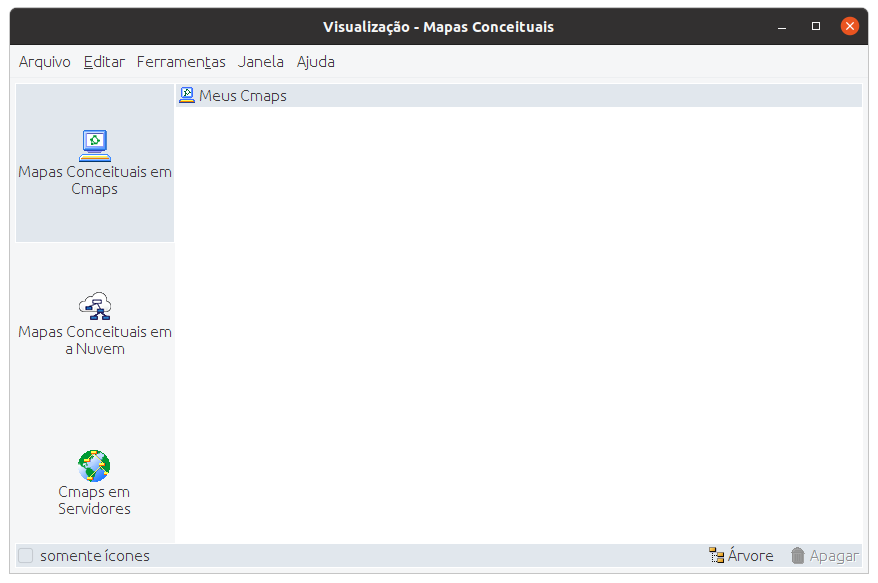
\includegraphics[scale=0.4]{cap05/InstCMap.png}
\caption{instalação do CmapTools}
\end{figure}

Porém observe que no Dash não aparece nenhum novo aplicativo, então precisamos criar um lançador. Utilizar o seguinte conteúdo:
\begin{lstlisting}
[Desktop Entry]
Name=CMapTools
Comment=Editor de Mapas Conceituais
Exec=/home/fernando/'IHMC CmapTools'/bin/CmapTools
Icon=/home/fernando/IHMC CmapTools/cmap-logo.png
Terminal=false
Type=Application
StartupNotify=true
Categories=Office
Keywords=Mapa;Conceitual;Editor;Conceptual;
\end{lstlisting}

\section{Ambiente de Programação Java}\index{Instalações fora dos padrões}
\textbf{Java} é atualmente a principal linguagem de programação, mais usada no mundo e com fortíssima empregabilidade (recebo uma média de 3 a 4 ofertas por dia de emprego nessa área). E não sou apenas eu que estou dizendo mas o \textbf{Instituto Tiobe}\footnote{Em: \url{https://www.tiobe.com/tiobe-index/}} então engole o choro com qualquer outra. Creio que Java ainda vai reinar supremo por muito tempo, pelo menos enquanto continuar sua alta capacidade de se adaptar aos ambientes mais heterogêneos.

\subsection{Editor Eclipse}\index{Instalações fora dos padrões}
Por enquanto neste mundo o Eclipse ainda é o principal editor utilizado pela grande maioria dos programadores, sua instalação é bem simples. Baixar o arquivo compactado no site oficial (em \url{http://www.eclipse.org}). Recomendo a versão ``Eclipse IDE for Java EE Developers'' para trabalhar. Após o download, descompacte-o na pasta /Downloads mesmo, observe que na pasta criada foi criada uma subpasta /eclipse. Pulemos então para o terminal.

O ideal é que o Eclipse seja instalado em uma pasta disponível para qualquer usuário do sistema, esta pasta é a /opt, então vamos acessá-la: \\
{\ttfamily\$ cd /opt}

Trazer o aplicativo para esta pasta: \\
{\ttfamily\$ mv $\sim$/eclipse-jee-[versão]/eclipse/ .}

Pronto está instalado, agora o próximo passo é criar um lançador para o Dash. Utilizar o seguinte conteúdo:
\begin{lstlisting}
[Desktop Entry]
Name=Eclipse
Comment=Ferramenta de Desenvolvimento Java
Exec=/opt/eclipse/eclipse
Icon=/opt/eclipse/icon.xpm
Terminal=false
Type=Application
Categories=Deploy
Keywords=IDE;Desenvolvimento;Java;Editor;
\end{lstlisting}

\subsection{Wildfly}\index{Instalações fora dos padrões}
Junto com o Eclipse precisamos de um servidor de aplicações ``Java EE'', antigamente seu nome era JBoss, mas foi modificado para Wildfly. Baixar o arquivo compactado no site oficial (em \url{http://wildfly.org}). Criamos uma pasta para conter os arquivos de trabalho, por exemplo: /Aplicativos. Descompactar o arquivo nesta pasta. E pronto está instalado.

\subsection{Git}\index{Instalações fora dos padrões}
Próximo passo e instalar um repositório de arquivos, o padrão Git é o melhor que conheço e se adapta facilmente ao Linux. Para instalá-lo uma única linha e necessária: \\
{\ttfamily\$ sudo apt install git}

Para usá-lo configuraramos um usuário e o email cadastrado no site: \\
{\ttfamily\$ git config ---global user.name [seuUsuario] \\
\$ git config ---global user.email [seuEmail]}

\section{Programas em Java}\index{Instalações fora dos padrões}
Para quem desconhece o arquivos \textbf{.jar} são ``executáveis'' do Java. Na verdade trata-se apenas de um arquivo compactado com um pequeno detalhe a mais, um arquivo texto chamado \textbf{MANIFEST.MF}, só isso, nada de especial, sem magia negra ou pacto com alguma entidade ``microsoftliana''. Nesta seção vamos instalar alguns deles que considero bem práticos.

\subsection{FinanX, um clone da HP-12C}\index{Instalações fora dos padrões}
Quem conhece a calculadora HP-12C não abre mão, comprei uma quando ainda estava na Faculdade de TI e até hoje a utilizo para tudo. Existe um clone muito bom chamado FinanX e é um aplicativo criado em linguagem Java. Não existe instalação, basta baixar o arquivo compactado (no endereço \url{http://sourceforge.net/projects/finanx/}, descompactar e usar o seguinte comando no terminal: \\
{\ttfamily\$ java -jar finanx.jar}

Que o aplicativo será chamado. Até aí tudo bonito, mas o ideal seria chamá-lo através do Dash e poder acessá-lo quando quiser. Primeiro vamos criar uma pasta, abaixo da /opt para receber os arquivos: \\
{\ttfamily\$ cd /opt \\
\$ sudo mkdir HP12C}

Entrar nesta pasta: \\
{\ttfamily\$ cd HP12C/}

E trazer os arquivos necessários (considerando que foram descompactados abaixo da pasta Downloads/ do seu usuário) para execução do programa: \\
{\ttfamily\$ sudo mv $\sim$/Downloads/finanx-12c[versao]/finanx.jar . \\
\$ sudo mv $\sim$/Downloads/finanx-12c[versao]/finanx.sh .}

Feito isso o próximo passo é criar um lançador para o Dash (busque um ícone na Internet e coloque nesta pasta) com o seguinte conteúdo:
\begin{lstlisting}
[Desktop Entry]
Name=HP12C
Comment=Calculadora HP12C
Exec=java -jar /opt/HP12C/finanx.jar
Icon=/opt/HP12C/hp_12C_Platinum_icon.png
Terminal=false
Type=Application
Categories=Office
Keywords=Calculadora;HP12C;Java;
\end{lstlisting}

\subsection{VUE, uma alternativa a Mapas Conceituais}\index{Instalações fora dos padrões}
Outro aplicativo distribuído na forma de .jar é o VUE desenvolvido pela \textbf{Universidade Tufts} e possui como objetivo principal é a criação de mapas de informação, que através de hiperligações, integra diferentes tipos de recursos como áudio, vídeo e imagens. Buscando desta forma facilitar a criação de materiais de apoio para o ensino e a aprendizagem através da utilização de recursos visuais.
\begin{figure}[H]
\centering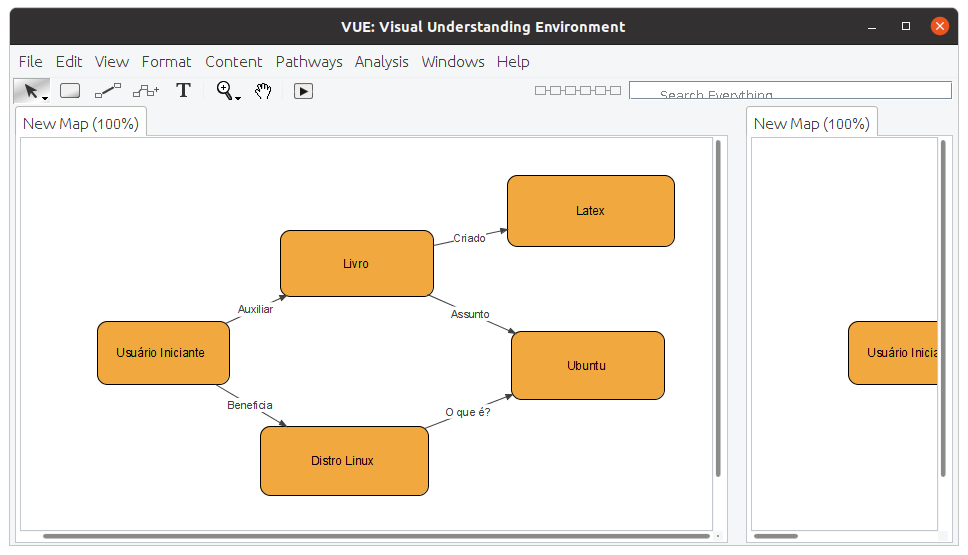
\includegraphics[scale=0.4]{cap05/Vue.png}
\caption{Mapa com o VUE}
\end{figure}

Para instalar faça o download da última versão disponível no site: \url{https://vue.tufts.edu} - Use a versão ``Linux / Generic JAR-only version''. Baixar o arquivo, copiar a pasta para /opt: \\
{\ttfamily\$ cd /opt \\
\$ sudo mkdir VUE \\
\$ cd VUE/ \\
\$ sudo mv $\sim$/Downloads/VUE.jar .}

Criar um lançador para o Dash (busque um ícone na Internet e coloque nesta pasta) com o seguinte conteúdo:
\begin{lstlisting}
[Desktop Entry]
Name=VUE
Comment=Ferramenta de Mapa Contextual
Exec=java -jar /opt/VUE/VUE.jar
Icon=/opt/VUE/visual-understanding-environment.jpg
Terminal=false
Type=Application
Categories=Deploy
Keywords=Mapa;Java;Editor;
\end{lstlisting}

\section{Compartilhando informações}\index{Instalações fora dos padrões}
Possuo duas máquinas desktop e notebook, a melhor forma de trocar informações entre elas é através de uma conexão SSH, então considere a seguinte nomenclatura: \vspace{-1em}
\begin{itemize}[noitemsep]
 \item Serv | Desktop local no cabeamento de rede (com o IP: XXX.XXX.SS.S) 
 \item Note | Notebook na WiFi (na mesma rede)
\end{itemize}

Note | Instalar o SSH: \\
{\ttfamily\$ sudo apt install ssh}

Note | Criar uma pasta de montagem: \\
{\ttfamily\$ sudo mkdir /mnt/r3d3}

Note | Dar permissão a pasta para o usuário local: \\
{\ttfamily\$ sudo chmod -R 777 /mnt/r3d3}

Serv | Criar uma pasta de ligação: \\
{\ttfamily\$ mkdir ~/partilhar}

Serv | Instalar o SSH-Server: \\
{\ttfamily\$ sudo apt install openssh-server}

Note | Realizar a ligação: \\
{\ttfamily\$ sshfs fernando@XXX.XXX.SS.S:/home/fernando/partilhar /mnt/r3d3}

\section{Latex - Simplesmente Genial}\index{Instalações fora dos padrões}
Se já cruzou a fronteira do vestibular e teve de fazer algum trabalho acadêmico, pode ter sofrido em relação a formatação de seu documento. Não importa se a pessoa frequente graduação, especialização, mestrado, doutorado ou espera escrever um simples artigo acadêmico para uma revista técnica. A formatação de documentos acadêmicos costuma representar grandes dores de cabeça.

Para resolver esses problemas foi criado a linguagem TeX\footnote{O nome corresponde às primeiras letras da palavra “tecnologia” em grego} no final dos anos 70 por \textbf{Donald Knuth} para a Universidade de Stanford. LaTeX é um sistema tipográfico, usado para produzir documentos científicos e matemáticos que necessitam de grande qualidade tipográfica. É possível produzir todo o tipo de documento, desde cartas a livros. O LaTeX usa a TeX como sistema de formatação.

Latex é uma das melhores linguagens de edição já inventadas, não estou sofrendo de amores por ela, estou completamente apaixonado. Sem ela não teria este livro (talvez teria sim, mas a primeira versão que criei com o LibreOffice no qual a manutenção estava se tornando impraticável). A descobri no meio acadêmico, de tão versátil uso-a para criar vários trabalhos que desejo publicar (como microlivros na Academia\footnote{Em \url{http://cetrex.academia.edu/FernandoAnselmo}}, até meu Currículo está escrito neste formato.

Podemos usar qualquer editor para produzir arquivos nesta linguagem, minha recomendação foi dada no capítulo anterior. Além do editor precisamos também do pacote \textbf{abntex} que é utilizado as regras da ABNT e do \textbf{Okular}, um visualizador de documentos PDF. Para realizar a instação desses pacotes digite o seguinte comando: \\
{\ttfamily\$ sudo apt install abntex okular tex-common}

Todos meus documentos que publico são produzidos com o LaTex e já se tornou algo que não consigo ficar sem, porém para usá-lo acabei me tornando dependente dos seguintes pacotes: \\
{\ttfamily\$ sudo apt-get install texlive-latex-extra \\
\$ sudo apt install texlive-lang-portuguese \\
\$ sudo apt-get install texlive-bibtex-extra \\
\$ sudo apt-get install texlive-games}

Para começar a produzir seus documentos recomendo baixar uma apostila intitulada \textbf{Uma não tão pequena introdução ao LaTeX}\footnote{Pode ser encontrada em http://tug.ctan.org/info/lshort/portuguese/pt-lshort-a5.pdf}.

\section{cURL um FTP diferente}\index{Instalações fora dos padrões}
O cURL e uma ferramenta exclusivamente usada no terminal para manipulação de URLs e transferência de dados. O principal benefício do cURL é que pode ser usado em arquivos shell scripts para automatizar a manipulação de URL. Suporta protocolos, como: FTP, HTTP, FTPS, TELNET, IMAP e outros.

Em termos simplificados, o cURL executa várias solicitações de um cliente para um servidor estabelecendo uma conexão por meio de um protocolo específico e seus métodos associados. Por exemplo, através de um cliente HTTP pode enviar um pedido para ler ou fazer download de conteúdo (método de solicitação GET), ou postar conteúdo através de um formulário em um site (método de solicitação POST). Muitas aplicações e serviços web usam o cURL para interagir com suas interfaces.

Instalar: \\
{\ttfamily\$ sudo apt install curl}

Mostrar o tempo: \\
{\ttfamily\$ curl http://wttr.in/BRASILIA}

Mostrar a fase da lua: \\
{\ttfamily\$ curl http://wttr.in/Moon}

Meu site FTP: \\
{\ttfamily\$ curl -u [usuario]:[senha] ftp://[end.FTP]}

Obter arquivos via FTP: \\
{\ttfamily\$ curl -O http://[end.Pág]}

Enviar um arquivo via FTP: \\
{\ttfamily\$ curl -T [arquivo] -u [usuario]:[senha] ftp://[end.FTP]/[pasta Local]/[arquivo]}

\section{Conky, informações na Área de Trabalho}\index{Instalações fora dos padrões}
Conky é um monitor do sistema bem leve e está disponível tanto para o Linux quanto para o BSD. Ter sempre a mão detalhes como temperatura, uso de CPU, RAM, rede, disco e a área de troca pode ser mais simples que você imagina, além disso exibir todas as informações do sistema e estatísticas de uma maneira elegante Essa maravilha é bem simples (basta tomar alguns cuidados básicos). \\[3mm]
Para instalar apenas digite no terminal o comando: \\
{\ttfamily\$ sudo apt install conky-all}

Agora vamos para a configuração, no Nautilus crie uma pasta na /home do seu usuário com o nome de .conky, porém quando concluir a ação ela desaparecerá, não se assuste no Linux os arquivos ou pastas escondidas são iniciadas por ``.'' para torná-la visível novamente pressione Ctrl + H.

Nesta pasta precisamos criar um arquivo, porém observe que clicando com o botão direito do mouse não aparece uma opção para se criar um documento, chame o gEdit no bash e salve um arquivo vazio (qualquer nome a sua escolha, mas o ideal é ``Novo Arquivo'') na pasta \textbf{Modelos}. Retorne a pasta .conky e clique com o botão direito novamente e observe que apareceu a opção
\textbf{Novo Documento}, crie um documento chamado \textbf{meutema} com o seguinte conteúdo:
\begin{lstlisting}
conky.config = {
  background=true,
  update_interval=5,
  double_buffer=false,
  no_buffers=true,
  text_buffer_size=2048,
  override_utf8_locale=true,
  use_xft=true,
  uppercase=false,
  gap_x=15,
  gap_y=80,
  minimum_size=300,
  maximum_width=350,
  own_window=true,
  own_window_type='normal',
  own_window_transparent=true,
  own_window_argb_visual=true,
  own_window_colour='000000',
  own_window_argb_value=38,
  own_window_hints='undecorated,below,sticky,skip_taskbar,skip_pager',
  border_inner_margin=0,
  border_outer_margin=0,
  alignment='top_right',
  draw_shades=false,
  draw_outline=false,
  draw_borders=false,
  draw_graph_borders=false,
  default_color='#000000',
  color0='#FFFFFF',
  color1='#EDE987',
  color2='#D3D3Ef',
  color3='#C7C7DB',
  color4='#EDE987',
  color5='#EDE987'
};
conky.text = [[
  ${font Ubuntu:bold:size=10}${color4}SISTEMA ${hr 2}
  ${voffset 2}
  ${offset 15}${font Ubuntu:size=10}${color1}$nodename
  ${offset 15}${font Ubuntu:size=10}${color1}$sysname Kernel: ${color0}$kernel
  ${offset 15}${font Ubuntu:size=10}${color1}Boot: ${color0}$uptime

  ${offset 15}${color4}SWAP: ${color0}$swapperc% ($swap/$swapmax)
  ${offset 15}${color3}${swapbar 5,150}

  ${offset 15}${font Ubuntu:bold:size=10}${color5}CPU
  ${offset 15}${cpugraph 40,285 AAAAAA 666666}
 
  ${voffset 2}
  ${offset 15}${font Ubuntu:bold:size=10}${color5}Consumo CPU
  ${offset 35}${font Ubuntu:size=10}${color4}${top name 1}${alignr}${top cpu 1}%
  ${offset 35}${font Ubuntu:size=10}${color1}${top name 2}${alignr}${top cpu 2}%
  ${offset 35}${font Ubuntu:size=10}${color2}${top name 3}${alignr}${top cpu 3}%
  ${offset 35}${font Ubuntu:size=10}${color3}${top name 4}${alignr}${top cpu 4}%
  ${offset 35}${font Ubuntu:size=10}${color3}${top name 5}${alignr}${top cpu 5}%
  ${offset 35}${font Ubuntu:size=10}${color3}${top name 6}${alignr}${top cpu 6}%

  ${voffset 2}
  ${offset 15}${font Ubuntu:bold:size=10}${color5}Consumo Memoria
  ${offset 35}${font Ubuntu:size=10}${color4}${top_mem name 1}${alignr}${top_mem mem 1}%
  ${offset 35}${font Ubuntu:size=10}${color1}${top_mem name 2}${alignr}${top_mem mem 2}%
  ${offset 35}${font Ubuntu:size=10}${color2}${top_mem name 3}${alignr}${top_mem mem 3}%
  ${offset 35}${font Ubuntu:size=10}${color3}${top_mem name 4}${alignr}${top_mem mem 4}%
  ${offset 35}${font Ubuntu:size=10}${color3}${top_mem name 4}${alignr}${top_mem mem 5}%

  ${voffset 2}
  ${offset 15}${font Ubuntu:bold:size=10}${color5}DISCOS
  ${offset 15}${diskiograph 40,285 AAAAAA 666666}
  ${voffset 2}
  ${offset 15}${font Ubuntu:bold:size=9}${color1}Livre: ${color0}${font Ubuntu:size=9}${fs_free}${alignr}${font Ubuntu:bold:size=9}${color1}Usada: ${color0}${font Ubuntu:size=9}${fs_used}

  ${voffset 2}
  ${offset 15}${font Ubuntu:bold:size=10}${color5}ETHERNET
  ${voffset 2}   
  ${offset 15}${font Ubuntu:size=9}${color1}Endereco IP: ${color0}${addr enp1s0}          
  ${voffset 2}   
  ${offset 15}${color1}${font Ubuntu:bold:size=9}Upload: ${alignr}${font Ubuntu:size=9}$color2${upspeed enp1s0} de ${totalup enp1s0}
  ${offset 15}${upspeedgraph enp1s0 40,285 AAAAAA 666666 100 -l}
  ${offset 15}${color1}${font Ubuntu:bold:size=9}Download: ${alignr}${font Ubuntu:size=9}$color2${downspeed enp1s0} de ${totaldown enp1s0}
  ${offset 15}${downspeedgraph enp1s0 40,285 AAAAAA 666666 100 -l}
  ${color4}${hr 2}
]];
\end{lstlisting}

Não, esse arquivo não é um monstro e não é tão complicado assim de se entender sua função é criar uma barra lateral com várias informações instantâneas. Agora para executá-lo precisamos dar o comando: \\
{\ttfamily\$ conky -c /home/[seuUsuario]/.conky/meutema}

Porém toda vez que desligar o computador essa barra desaparecerá e terá que repetir o comando no terminal, para evitar isso e torná-la permanente localize no Dash por ``Aplicativos Iniciais''. \vspace{-1em}
\begin{itemize}[noitemsep]
 \item Nome: Concky
 \item Comando: conky -c /home/[seuUsuario]/.conky/meutema
 \item Comentário: Execução do Conky
\end{itemize}

E agora é essa a provável aparência do seu desktop:
\begin{figure}[H]
	\centering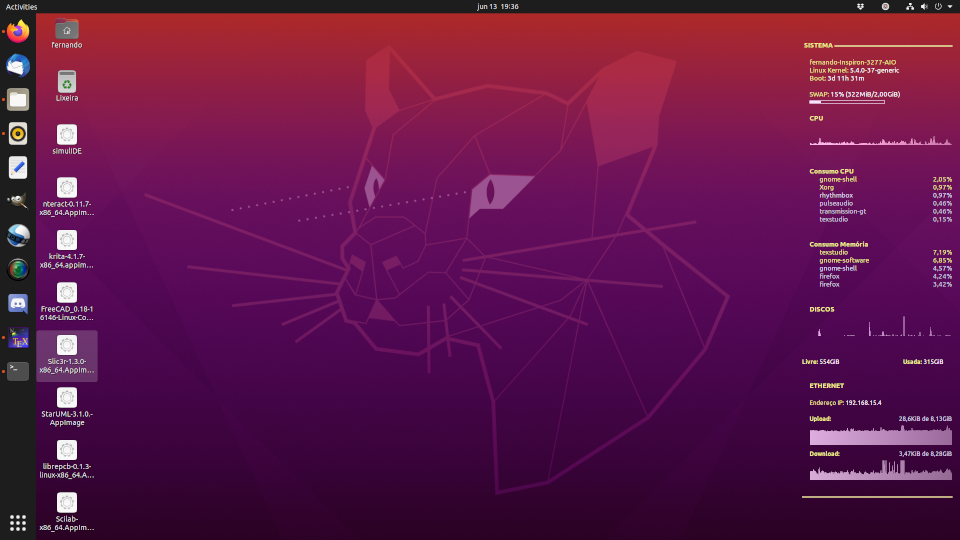
\includegraphics[scale=0.4]{cap05/MeuDesktop.png}
	\caption{Meu Desktop}
\end{figure}

Provável pois tenho uma terrível mania de ficar mudando meu papel de parede ou os comandos do Conky para me fornecer mais informações. E pensava que só usuário do Windows podia fazer isso?

% Final do Capítulo
\clearpage